% A Field Guide to Finite Element Families
% Build with:  latexmk -pdf finite_elements_guide.tex
% Figures are produced by figures/make_figures.py

\documentclass[11pt,a4paper]{article}

\usepackage[T1]{fontenc}
\usepackage[utf8]{inputenc}
\usepackage{mathptmx}
\usepackage[scaled=0.90]{helvet}
\usepackage{amsmath,amssymb}
\usepackage{microtype}
\usepackage{graphicx}
\usepackage{booktabs}
\usepackage{array}
\usepackage{enumitem}
\usepackage{caption}
\usepackage{xcolor}
\usepackage[most]{tcolorbox}
\usepackage{titlesec}
\usepackage{placeins}
\usepackage[a4paper,margin=2.6cm,top=2.4cm,bottom=2.6cm]{geometry}
\usepackage[hidelinks]{hyperref}

\graphicspath{{figures/}}

% ---------------------------------------------------------------- colours --
\definecolor{cH1}{HTML}{2F5FA8}
\definecolor{cHcurl}{HTML}{7A4FA3}
\definecolor{cHdiv}{HTML}{C0562A}
\definecolor{cL2}{HTML}{1A7F64}
\definecolor{cCR}{HTML}{8A6D1F}
\definecolor{cInk}{HTML}{22242A}
\definecolor{cDim}{HTML}{6B6F7A}
\definecolor{cWarn}{HTML}{B3243C}

\hypersetup{
  colorlinks=true, linkcolor=cH1, urlcolor=cHdiv, citecolor=cH1,
  pdftitle={A Field Guide to Finite Element Families},
  pdfsubject={Lagrange, discontinuous Galerkin, Raviart-Thomas, BDM and Nedelec elements},
}

% ------------------------------------------------------------- structuring --
\titleformat{\section}{\normalfont\sffamily\Large\bfseries\color{cInk}}{\thesection}{0.8em}{}
\titleformat{\subsection}{\normalfont\sffamily\large\bfseries\color{cInk}}{\thesubsection}{0.7em}{}
\titleformat{\subsubsection}{\normalfont\sffamily\normalsize\bfseries\color{cDim}}{}{0em}{}
\titlespacing*{\section}{0pt}{1.9\baselineskip}{0.7\baselineskip}
\titlespacing*{\subsection}{0pt}{1.3\baselineskip}{0.45\baselineskip}

\captionsetup{font=small,labelfont={bf,sf},labelsep=period,width=0.95\textwidth}

% let figures take up more of a page, so fewer half-empty pages appear
\renewcommand{\topfraction}{0.92}
\renewcommand{\bottomfraction}{0.75}
\renewcommand{\textfraction}{0.08}
\renewcommand{\floatpagefraction}{0.78}
\setcounter{topnumber}{3}
\setcounter{bottomnumber}{2}
\setcounter{totalnumber}{4}

\setlist[itemize]{topsep=3pt,itemsep=2pt,parsep=0pt,leftmargin=1.35em}
\setlist[enumerate]{topsep=3pt,itemsep=2pt,parsep=0pt,leftmargin=1.6em}
\setlist[description]{topsep=3pt,itemsep=3pt,parsep=0pt,leftmargin=0pt,
                      font=\normalfont\sffamily\bfseries\small}

% ------------------------------------------------------------------ boxes --
\newtcolorbox{jargon}[1]{%
  enhanced, breakable, colback=black!3, colframe=black!22, boxrule=0.5pt,
  arc=2pt, left=8pt, right=8pt, top=5pt, bottom=6pt,
  fonttitle=\sffamily\bfseries\small, coltitle=cInk, colbacktitle=black!9,
  title={#1}, attach boxed title to top left={xshift=8pt,yshift=-2pt},
  boxed title style={boxrule=0pt, colframe=black!9, arc=1pt}}

\newtcolorbox{keypoint}[1][cInk]{%
  enhanced, breakable, colback=#1!4, colframe=#1, boxrule=0pt, leftrule=2.6pt,
  arc=0pt, outer arc=0pt, left=9pt, right=9pt, top=6pt, bottom=6pt}

% ------------------------------------------------------------------ macros --
\newcommand{\Hdiv}{H(\mathrm{div})}
\newcommand{\Hcurl}{H(\mathrm{curl})}
\newcommand{\dv}{\operatorname{div}}
\newcommand{\curl}{\operatorname{curl}}
\newcommand{\jump}[1]{[\![#1]\!]}
\newcommand{\avg}[1]{\{\!\{#1\}\!\}}
\newcommand{\dx}{\,\mathrm{d}x}
\newcommand{\ds}{\,\mathrm{d}s}
\newcommand{\bn}{\mathbf{n}}
\newcommand{\bt}{\mathbf{t}}
\newcommand{\bu}{\mathbf{u}}
\newcommand{\bv}{\mathbf{v}}
\newcommand{\bx}{\mathbf{x}}
\newcommand{\bE}{\mathbf{E}}
\newcommand{\Th}{\mathcal{T}_h}
\newcommand{\RR}{\mathbb{R}}
\newcommand{\spaceH}[1]{\textcolor{#1}{\bfseries}}

\newcommand{\cH}[1]{\textcolor{cH1}{#1}}
\newcommand{\cC}[1]{\textcolor{cHcurl}{#1}}
\newcommand{\cD}[1]{\textcolor{cHdiv}{#1}}
\newcommand{\cL}[1]{\textcolor{cL2}{#1}}

\begin{document}

% ============================================================== title page ==
\begin{titlepage}
\centering
\vspace*{3.4cm}

{\sffamily\fontsize{13}{16}\selectfont\color{cDim}
 A VISUAL INTRODUCTION\par}

\vspace{0.9cm}
{\sffamily\fontsize{30}{36}\selectfont\bfseries\color{cInk}
 A Field Guide to\\[0.18em] Finite Element Families\par}

\vspace{1.1cm}
{\fontsize{13}{18}\selectfont\color{cDim}
 Why there is more than one kind of finite element,\\
 and how to tell them apart\par}

\vspace{1.8cm}
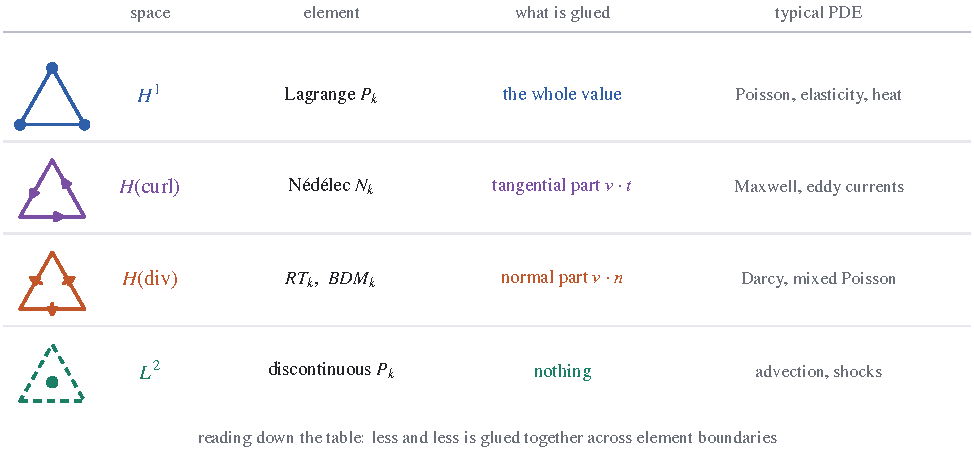
\includegraphics[width=0.99\textwidth]{fig_cheatsheet.pdf}

\vfill
{\small\color{cDim}
 Companion notes to the \texttt{falk-mixed-elasticity} repository.\\
 Everything in this document is reproducible: see \texttt{README.md}.\par}
\vspace{0.6cm}
\end{titlepage}

% ================================================================= preface ==
\section*{Before you start}
\addcontentsline{toc}{section}{Before you start}

This guide is written for someone who is comfortable with calculus and linear
algebra --- gradients, divergence, integration by parts, vector spaces, bases
--- but who has never sat down and studied finite element spaces. You do not
need to have met Sobolev spaces, weak formulations or the \emph{inf-sup}
condition before; each of those is introduced here when it is first needed,
in plain language before any notation appears.

The question the guide answers is this one:

\begin{keypoint}
Software like FEniCSx offers you \texttt{Lagrange}, \texttt{DG},
\texttt{RT}, \texttt{BDM}, \texttt{N1curl} and a dozen more. Why are there so
many? What actually distinguishes them, and how do you know which one your
equation wants?
\end{keypoint}

\noindent The short answer, which the rest of the guide unpacks, is that the
families differ in \textbf{how much of a function is forced to match across
the boundary between two neighbouring cells} --- and that the right amount of
matching is dictated by the partial differential equation you are solving, not
by taste.

One practical note on reading: almost every diagram in this guide shows the
\emph{same} two triangles meeting along one edge. That is deliberate. Once you
have the picture of two cells and their shared edge in your head, every element
family becomes a different answer to the single question ``what happens on that
edge?''.

\vspace{0.6em}
\noindent\textcolor{cDim}{\small A note on indices: this guide uses the classical
mathematical convention in which $RT_0$ and $N_0$ denote the \emph{lowest-order}
Raviart--Thomas and Nédélec spaces. Some software, including Basix/FEniCSx,
counts from one instead, so the lowest-order space is called degree~1 there.
The elements are the same; only the label shifts by one.}

\tableofcontents
\newpage

% =================================================================== \S 1 ==
\section{What is a finite element?}

Suppose you want to solve a partial differential equation on some region
$\Omega$ --- the temperature in a turbine blade, the pressure in an aquifer,
the electric field in a waveguide. The unknown is a function, and a function
carries infinitely much information. A computer needs finitely many numbers.
The finite element method is one recipe for choosing which finitely many
numbers to keep.

The recipe has three ingredients, and it is worth separating them carefully,
because almost all the variety between element families lives in the third one.

\subsection{Ingredient one: the mesh}

Chop $\Omega$ into small, simple pieces: triangles or quadrilaterals in two
dimensions, tetrahedra or hexahedra in three. Call the collection $\Th$, an
individual piece a \emph{cell} or \emph{element}, and write $h$ for the typical
cell diameter. The pieces must fit together exactly --- no gaps, no overlaps,
and (for the standard theory) a vertex of one triangle may not land in the
middle of another triangle's edge.

Two cells that share an edge are \emph{neighbours}, and the edge they share is
called a \emph{facet} (an edge in 2D, a triangular face in 3D). Facets are
where all the interesting behaviour happens.

\begin{figure}[htbp]
\centering
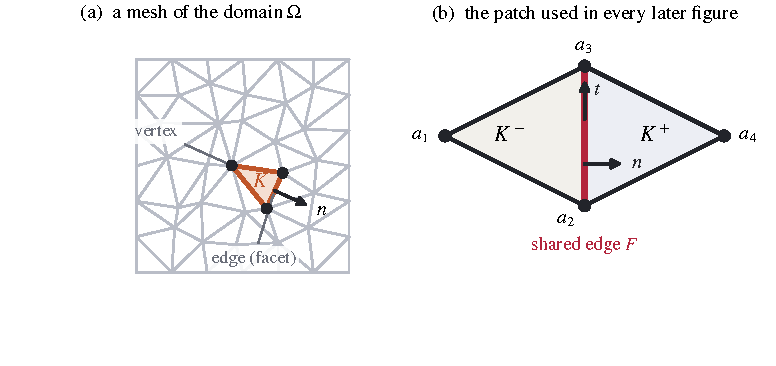
\includegraphics[width=\textwidth]{fig_mesh.pdf}
\caption{Left: a mesh of a square domain, with one cell $K$ highlighted and the
outward unit normal $\bn$ on one of its edges. Right: the two-cell patch that
every later figure in this guide reuses. The shared edge $F$ carries a normal
direction $\bn$ (pointing across it) and a tangential direction $\bt$ (pointing
along it).}
\label{fig:mesh}
\end{figure}

\subsection{Ingredient two: a polynomial on each cell}

On each individual cell we approximate the unknown by a polynomial of low
degree. Two reasons make polynomials the natural choice. Practically, they are
trivial to differentiate and to integrate exactly by quadrature. Theoretically,
Taylor's theorem says that any smooth function looks like a polynomial of
degree $k$ when you zoom in far enough, with an error of size $O(h^{k+1})$ on a
cell of diameter $h$. So refining the mesh and raising the degree are two
different knobs for the same goal.

Write $P_k(K)$ for the polynomials of total degree at most $k$ on the cell $K$.
In two dimensions
\[
  P_1 = \operatorname{span}\{1,\;x,\;y\},\qquad
  P_2 = \operatorname{span}\{1,\;x,\;y,\;x^2,\;xy,\;y^2\},
\]
of dimension $3$ and $6$; in general $\dim P_k = \tfrac12 (k+1)(k+2)$ in 2D.

\subsection{Ingredient three: degrees of freedom}

Here is where the families separate. A polynomial on a cell is determined by
its coefficients, but coefficients are a terrible bookkeeping device: they have
no geometric meaning, and two neighbouring cells have no way to agree on them.
Instead we pin the polynomial down by \emph{degrees of freedom}.

\begin{jargon}{Degree of freedom}
A \emph{degree of freedom} (dof) is a rule that extracts one number from a
function. ``Its value at this vertex.'' ``Its average over this edge.'' ``The
flux of this vector field through this edge.'' Formally it is a linear
functional. A set of dofs is good if it is \emph{unisolvent}: knowing all the
numbers determines the polynomial uniquely.
\end{jargon}

For $P_1$ on a triangle, the classical choice is the value at each of the three
vertices. Three numbers, three dimensions, and a linear function in the plane is
indeed fixed by its values at three non-collinear points --- unisolvent.

\begin{figure}[htbp]
\centering
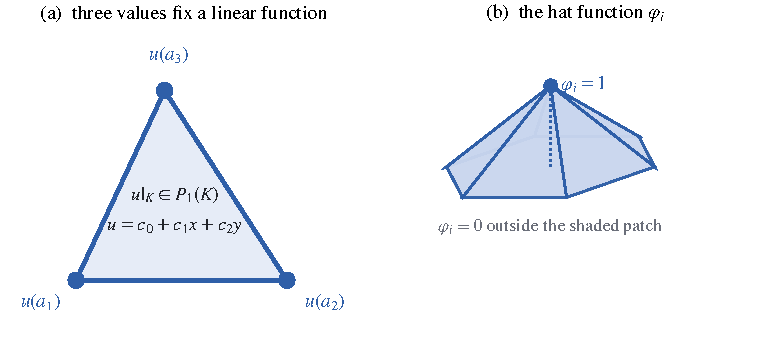
\includegraphics[width=\textwidth]{fig_p1_dofs.pdf}
\caption{Left: the three degrees of freedom of the $P_1$ Lagrange triangle.
Right: the corresponding global basis function, the ``hat'' $\varphi_i$, which
equals~$1$ at one vertex, $0$ at every other vertex, and vanishes outside the
cells touching that vertex. Small support is what makes the resulting matrices
sparse.}
\label{fig:p1dofs}
\end{figure}

The formal definition, due to Ciarlet, packages exactly these three ingredients:
a finite element is a triple $(K, P, \Sigma)$ --- a cell, a space of
polynomials on it, and a unisolvent set of dofs. When people say ``the
Raviart--Thomas element'' they mean a particular choice of $P$ and $\Sigma$.

\subsection{Assembling cells into a global space}

Now the step that matters most. We have a polynomial on every cell; we want one
function on all of $\Omega$. The rule is simple and it is the key to this whole
guide:

\begin{keypoint}[cWarn]
\textbf{Degrees of freedom that two neighbouring cells share are stored once.}
A dof sitting on a vertex or an edge belongs to \emph{every} cell touching that
vertex or edge, so all of them are forced to agree on it. A dof sitting strictly
inside a cell belongs to that cell alone, and no neighbour ever sees it.
\end{keypoint}

That single bookkeeping decision --- where you attach the dofs --- determines
what is continuous across facets, and therefore which global function space you
end up in. Put the dofs on vertices and you glue values together. Put them on
edges and you glue something edge-related together. Put them strictly inside
and you glue nothing.

The rest of this guide is, quite literally, a catalogue of the different answers
to ``what do we glue?''.

Finally, a bookkeeping payoff: because each dof is shared by only a handful of
cells, the corresponding basis function (Figure~\ref{fig:p1dofs}, right) is
nonzero only on those few cells. Two basis functions whose supports do not
overlap contribute a zero to the stiffness matrix, so the matrix is sparse ---
which is the reason the method scales to millions of unknowns.

\FloatBarrier

% =================================================================== \S 2 ==
\section{Why there is more than one kind of element}

If gluing more is always safer, why not always glue everything? Because the
equation you are solving decides how much gluing is \emph{necessary}, and
gluing more than necessary is at best wasteful and at worst simply wrong.

\subsection{Different equations, different unknowns}

The unknowns in real problems are not all scalar fields:

\begin{description}
\item[Scalar fields.] Temperature, pressure, concentration, electrostatic
  potential. One number per point.
\item[Vector fields.] Displacement of an elastic body, fluid velocity, electric
  and magnetic fields. Several numbers per point --- and, crucially, the
  components may not all behave the same way.
\item[Fluxes.] The Darcy velocity in a porous rock, the heat flux in a
  composite. These are vector fields whose entire physical meaning is ``how
  much stuff crosses this surface per unit time''.
\item[Tensor fields.] The stress in a solid. In the companion repository to
  this guide, the stress is the primary unknown.
\item[Quantities that genuinely jump.] The density across a shock wave, the
  concentration across a contact discontinuity. Forcing these to be continuous
  is not conservative caution --- it is a modelling error.
\end{description}

\subsection{Weak formulations, and why they decide everything}

Finite elements do not solve the PDE pointwise. They solve its \emph{weak} (or
variational) form.

\begin{jargon}{Weak formulation}
Multiply the equation by an arbitrary smooth \emph{test function} $v$,
integrate over $\Omega$, and use integration by parts to move derivatives off
the unknown and onto $v$. The result is a family of integral identities, one
per test function. A function satisfying all of them is a \emph{weak solution}.
The point is that integrals tolerate functions that are far less smooth than
the original PDE seems to require --- kinks, and sometimes jumps.
\end{jargon}

Take the Poisson equation $-\Delta u = f$. Multiply by $v$ vanishing on
$\partial\Omega$ and integrate by parts once:
\[
  \int_\Omega \nabla u \cdot \nabla v \dx \;=\; \int_\Omega f\, v \dx .
\]
Look at what survives: exactly one derivative on $u$, and it appears inside a
square-integrable pairing. So the natural home for $u$ is the set of functions
whose \emph{first derivatives are square-integrable}. That set has a name.

\begin{jargon}{The spaces $L^2$, $H^1$, $\Hdiv$, $\Hcurl$}
$L^2(\Omega)$ is the set of functions with $\int_\Omega u^2 < \infty$ --- finite
energy, no smoothness required at all. The others add exactly one derivative,
but only the derivative combination the PDE actually uses:
\[
\begin{array}{llll}
  H^1     &=\{u : u \in L^2,\ \nabla u \in L^2\}
          &\quad\text{\emph{all} first derivatives}\\[2pt]
  \Hdiv   &=\{\bv : \bv \in L^2,\ \dv \bv \in L^2\}
          &\quad\text{only the divergence}\\[2pt]
  \Hcurl  &=\{\bv : \bv \in L^2,\ \curl \bv \in L^2\}
          &\quad\text{only the curl}
\end{array}
\]
$\Hdiv$ and $\Hcurl$ are strictly \emph{larger} than $(H^1)^d$: they ask for
less, because the PDE asks for less.
\end{jargon}

\begin{jargon}{Conformity}
A discrete space $V_h$ is \emph{conforming} for a problem posed in $V$ if
$V_h \subset V$. Conformity is what lets you reuse the whole theory of the
continuous problem. The entire design effort behind $RT$, $BDM$ and Nédélec
elements goes into making piecewise polynomials land inside $\Hdiv$ or
$\Hcurl$, which --- as we are about to see --- is a statement about facets.
\end{jargon}

\subsection{The one calculation that explains all of it}

Here is the computation that generates the whole catalogue. Take a function
$u_h$ that is a nice polynomial inside each cell but may jump across facets, and
ask: what is its derivative, understood in the weak sense?

Integrate by parts cell by cell against a smooth test function $\varphi$ that
vanishes near $\partial\Omega$:
\[
  \int_\Omega u_h\, \partial_i \varphi \dx
  \;=\; \sum_{K \in \Th} \Big( -\int_K \partial_i u_h\, \varphi \dx
        \;+\; \int_{\partial K} u_h\, \varphi\, n_i \ds \Big).
\]
Every interior facet $F$ is visited twice, once from each side, with opposite
normals. Writing $u^-$ and $u^+$ for the two one-sided limits and
$\jump{u} := u^- - u^+$ for the \emph{jump}, the boundary terms collapse to
\begin{equation}\label{eq:ibp}
  \int_\Omega u_h\, \partial_i \varphi \dx
  \;=\; -\underbrace{\sum_{K}\int_K \partial_i u_h\, \varphi \dx}_{\text{the piecewise derivative}}
  \;+\; \underbrace{\sum_{F}\int_F \jump{u_h}\, \varphi\, n_i \ds}_{\text{a term living on the facets}} .
\end{equation}
The first term is an ordinary $L^2$ function. The second is not a function at
all: it is a measure concentrated on a surface, a Dirac delta smeared over the
facet. Its ``value'' is infinite on a set of zero volume.

\begin{figure}[htbp]
\centering
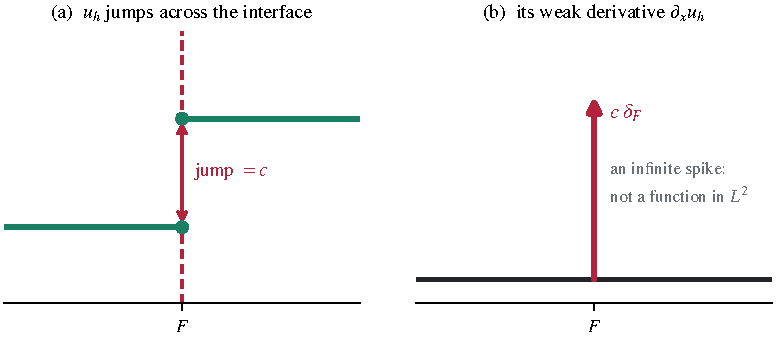
\includegraphics[width=\textwidth]{fig_jump_delta.pdf}
\caption{Why a jump throws you out of $H^1$. A piecewise constant function with
a jump of size $c$ across the facet $F$ has weak derivative equal to zero away
from $F$ plus an infinite spike of strength $c$ \emph{on} $F$. A spike is not a
square-integrable function, so the jumping function is not in $H^1$ --- no
matter how smooth it is inside each cell.}
\label{fig:jumpdelta}
\end{figure}

\noindent So, reading \eqref{eq:ibp} backwards:

\begin{keypoint}[cH1]
A piecewise polynomial lies in $H^1$ \textbf{if and only if} $\jump{u_h} = 0$
on every interior facet --- that is, if and only if it is continuous.
\end{keypoint}

\subsection{The same calculation for vector fields}

Now repeat it for the divergence. With $\bv_h$ piecewise polynomial and
$\varphi$ scalar,
\[
  \int_\Omega \bv_h \cdot \nabla \varphi \dx
  \;=\; -\sum_K \int_K (\dv \bv_h)\,\varphi \dx
  \;+\; \sum_F \int_F \jump{\bv_h \cdot \bn}\, \varphi \ds .
\]
Only the combination $\bv_h\cdot\bn$ appears. The tangential part of $\bv_h$
never enters. Hence:

\begin{keypoint}[cHdiv]
A piecewise polynomial vector field lies in $\Hdiv$ \textbf{if and only if} its
\emph{normal} component $\bv\cdot\bn$ is continuous across every facet. The
tangential component is free to jump.
\end{keypoint}

The curl version works the same way, using
$\nabla\cdot(\bv\times\varphi) = (\curl \bv)\cdot\varphi - \bv\cdot(\curl\varphi)$,
and produces the mirror-image conclusion:

\begin{keypoint}[cHcurl]
A piecewise polynomial vector field lies in $\Hcurl$ \textbf{if and only if} its
\emph{tangential} component is continuous across every facet. The normal
component is free to jump.
\end{keypoint}

\begin{figure}[htbp]
\centering
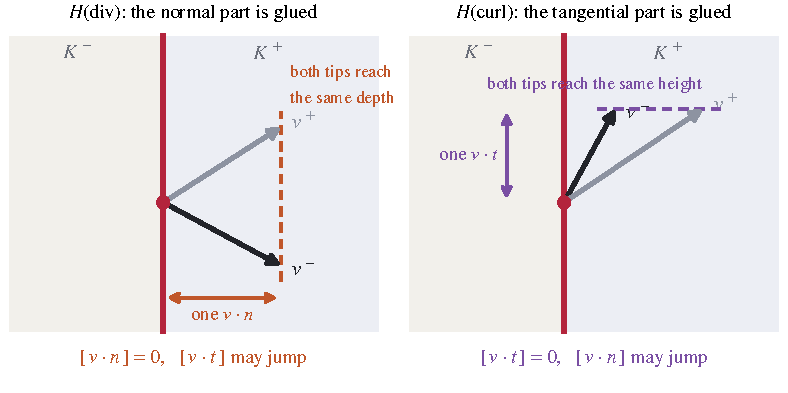
\includegraphics[width=\textwidth]{fig_normal_vs_tangential.pdf}
\caption{The central distinction of this guide. At a point on the shared edge,
a vector field has two one-sided limits, $\bv^-$ from the left cell and $\bv^+$
from the right. In an $\Hdiv$ field (left) the two arrows reach equally far
\emph{across} the edge --- the normal components agree --- while their
along-edge parts differ. In an $\Hcurl$ field (right) the two arrows reach
equally far \emph{along} the edge and differ across it. Neither field is
continuous as a vector; each is continuous in exactly one component.}
\label{fig:normvstan}
\end{figure}

\subsection{What this buys us}

Three observations close the section.

First, $H^1$-conformity is the \emph{strongest} of the three conditions: it
forces both components to match. $\Hdiv$ and $\Hcurl$ each force one. $L^2$
forces none. So $(H^1)^d \subset \Hdiv \cap \Hcurl$, and both of those sit
inside $L^2$.

Second, the conditions on $\Hdiv$ and $\Hcurl$ are not comparable with each
other. Neither is stronger. They are siblings.

Third --- and this is the practical punchline --- \emph{demanding more
continuity than the PDE needs is not a safe default}. It shrinks the space, so
it costs accuracy per unknown; and when the true solution genuinely has a jump
in the component you glued, it makes the method converge to the wrong answer.
Sections~\ref{sec:rt} and~\ref{sec:nedelec} both contain concrete instances.

\FloatBarrier

% =================================================================== \S 3 ==
\section{Lagrange elements: gluing the value}

\begin{keypoint}[cH1]
\textbf{Approximates:} a scalar field (or each component of a vector field
independently).\quad
\textbf{Dofs:} point values at nodes.\quad
\textbf{Continuous:} the whole value.\quad
\textbf{Lives in:} $H^1$.\quad
\textbf{Used for:} Poisson, heat, elasticity --- anything whose weak form
contains $\nabla u \cdot \nabla v$.
\end{keypoint}

\subsection{The element}

The Lagrange element of degree $k$ takes $P_k(K)$ on each cell and uses point
values at a lattice of nodes as its dofs:

\begin{itemize}
\item $P_1$: the 3 vertices.
\item $P_2$: the 3 vertices and the 3 edge midpoints --- 6 nodes, and
      $\dim P_2 = 6$.
\item $P_3$: 3 vertices, 2 points on each of the 3 edges, 1 interior point ---
      10 nodes, and $\dim P_3 = 10$.
\end{itemize}

The pattern generalises: vertices first, then interior-of-edge nodes, then
interior-of-face nodes, and so on.

\subsection{Why point values at shared nodes give continuity}

This is worth doing carefully once, because the argument recurs for every
family in a different guise.

Take $P_2$ and two triangles sharing an edge $F$. Restricted to $F$, a function
in $P_2$ of two variables becomes a polynomial of degree~2 in one variable ---
and a one-dimensional quadratic is determined by three values. The three nodes
sitting on $F$ (two endpoints plus the midpoint) supply exactly those three
values, and both cells are forced to use the same numbers. Therefore the two
traces on $F$ coincide identically, not merely at the nodes.

That is the mechanism in general: the dofs lying on a facet must be enough to
determine the \emph{trace} on that facet, and they must be shared.

\begin{figure}[htbp]
\centering
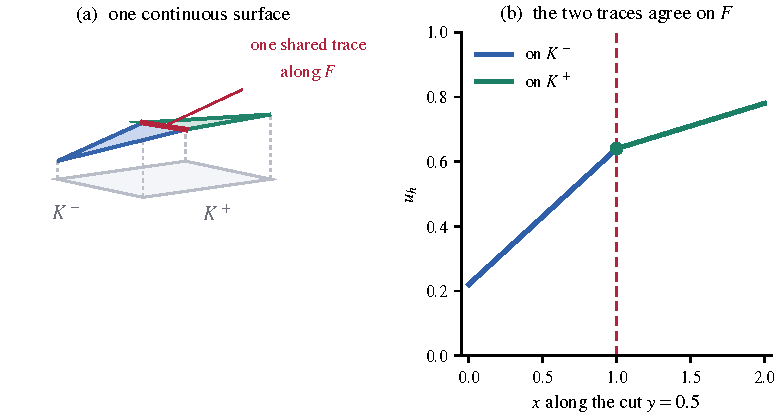
\includegraphics[width=\textwidth]{fig_lagrange_continuity.pdf}
\caption{A $P_1$ Lagrange function on the two-cell patch. The two triangles
share the values at both endpoints of the common edge, so the two linear traces
along that edge are the same function: the graph is a single unbroken surface.
Right: a cut through the patch. The function is continuous, but its slope is
not --- $C^0$, not $C^1$, which is exactly what $H^1$ asks for.}
\label{fig:lagrange}
\end{figure}

Note what the right-hand panel of Figure~\ref{fig:lagrange} also shows: the
derivative \emph{does} jump. That is fine. $H^1$ requires
$\nabla u \in L^2$, and a function with a finite jump in its slope has a
perfectly good bounded gradient --- the gradient jumps, but it never becomes a
spike. Only a jump in the \emph{value} produces the Dirac term of
Figure~\ref{fig:jumpdelta}.

\subsection{The model problem}

For $-\Delta u = f$ with $u = 0$ on the boundary, set
\[
  V_h = \big\{\, v_h \ \text{continuous, piecewise } P_k,\
                 v_h|_{\partial\Omega} = 0 \,\big\},
\]
and solve: find $u_h \in V_h$ with
\[
  \int_\Omega \nabla u_h \cdot \nabla v_h \dx = \int_\Omega f v_h \dx
  \qquad \text{for all } v_h \in V_h .
\]
Because $V_h \subset H^1_0$, this is a conforming method, and the classical
error estimates apply: for a smooth solution,
\[
  \|u - u_h\|_{H^1} = O(h^{k}), \qquad \|u - u_h\|_{L^2} = O(h^{k+1}).
\]

\subsection{The physical reading}

$H^1$-continuity is the mathematical statement of ``this quantity cannot jump''.
Temperature cannot jump across an imaginary surface drawn inside a solid.
Displacement cannot jump inside an intact material --- a jump would mean the
material has torn. When your unknown is a quantity of that kind, Lagrange
elements are not merely convenient; they encode the physics.

The flip side is the subject of the next four sections: when the unknown is
\emph{not} of that kind, Lagrange elements impose a constraint the physics does
not have.

\FloatBarrier

% =================================================================== \S 4 ==
\section{Discontinuous Galerkin: gluing nothing}

\begin{keypoint}[cL2]
\textbf{Approximates:} a scalar or vector field that may genuinely jump, or one
that is never differentiated.\quad
\textbf{Dofs:} cell-local, shared with nobody.\quad
\textbf{Continuous:} nothing.\quad
\textbf{Lives in:} $L^2$.\quad
\textbf{Used for:} conservation laws and transport; also as the ``other half''
of mixed methods.
\end{keypoint}

\subsection{The element}

Take the same $P_k$ polynomials as before --- and refuse to share anything. Each
cell carries its own independent copy, so the global dimension is simply
(number of cells) $\times \dim P_k$. Nothing links a cell to its neighbour.

The dofs are usually still point values at nodes, but the nodes are understood
as belonging to that cell alone. Two cells meeting at a vertex have two separate
values there, and nothing forces them to agree.

\begin{figure}[htbp]
\centering
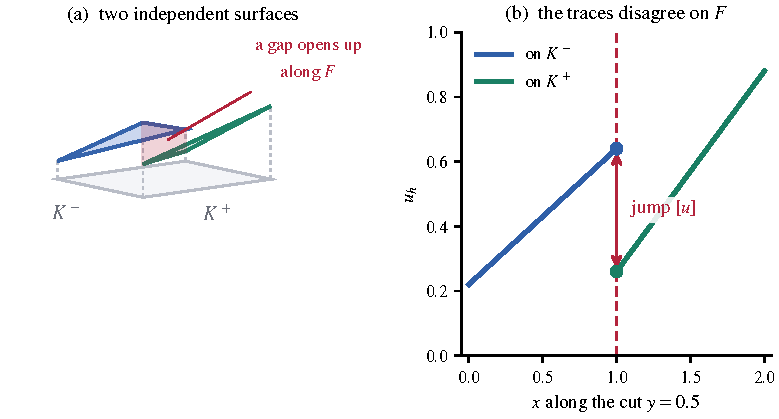
\includegraphics[width=\textwidth]{fig_dg_jump.pdf}
\caption{A discontinuous $P_1$ function on the same patch. The two cells now
carry unrelated linear functions, so the two traces along the shared edge
differ and the graph tears open. The size of the tear is the jump
$\jump{u_h} = u^- - u^+$, which for DG methods is not an error to be eliminated
but a quantity the method actively works with.}
\label{fig:dgjump}
\end{figure}

\subsection{If nothing is glued, what holds the solution together?}

A good question, and the answer is the defining idea of the method: the cells
are coupled \emph{through the equations}, not through the space. Since the
pieces do not agree at a facet, the method has to choose what value to use
there --- and that choice is called a \emph{numerical flux}.

\begin{jargon}{Jump, average, numerical flux}
On a facet with two one-sided limits $u^\pm$, define
$\jump{u} = u^- - u^+$ and $\avg{u} = \tfrac12(u^- + u^+)$.
A \emph{numerical flux} $\hat{u}$ is a single value, built from $u^-$ and $u^+$,
that both cells agree to use in place of the true trace. Different choices give
different methods.
\end{jargon}

For the transport equation $\partial_t u + \nabla\cdot(\mathbf{b}\,u) = 0$,
multiply by a test function supported on one cell and integrate by parts on
that cell alone:
\[
  \frac{\mathrm{d}}{\mathrm{d}t}\int_K u_h v \dx
  \;-\; \int_K u_h\, \mathbf{b}\cdot\nabla v \dx
  \;+\; \int_{\partial K} \hat{u}\, (\mathbf{b}\cdot\bn)\, v \ds \;=\; 0 .
\]
The natural choice for $\hat u$ is \emph{upwinding}: take the value from
whichever side the flow is coming from,
\[
  \hat u = \begin{cases} u^- & \text{if } \mathbf{b}\cdot\bn > 0,\\
                         u^+ & \text{if } \mathbf{b}\cdot\bn < 0.\end{cases}
\]
This is not a trick; it is the numerical statement that information in a
transport problem travels downstream. Taking the average instead
($\hat u = \avg{u}$) gives a scheme that is unstable, for the same reason that
central differencing is unstable for advection.

For elliptic problems one wants the discontinuities to be small, so an
\emph{interior penalty} term
\[
  \sum_{F} \frac{\sigma}{h} \int_F \jump{u_h}\, \jump{v_h} \ds
\]
is added to the formulation. It pushes the jumps towards zero as the mesh
refines without ever forbidding them outright: continuity is enforced
\emph{weakly} instead of being built into the space.

\subsection{Why anyone would want this}

\begin{itemize}
\item \textbf{Genuine discontinuities.} The solution of a nonlinear conservation
  law develops shocks in finite time even from smooth data. A continuous space
  cannot represent a shock and responds with spurious oscillations near it.
\item \textbf{Local conservation.} Taking $v \equiv 1$ on a single cell turns
  the DG equation into an exact statement that what flows in minus what flows
  out equals the change inside \emph{that cell}. Conservation holds cell by
  cell, not merely globally.
\item \textbf{A block-diagonal mass matrix.} Because no basis function is shared
  between cells, the mass matrix is block diagonal with one small block per
  cell, and can be inverted cell by cell. For explicit time-stepping this is a
  decisive advantage.
\item \textbf{Easy adaptivity.} Neighbouring cells need not use the same
  polynomial degree and meshes need not match across an interface, since nothing
  has to line up.
\end{itemize}

The cost is unknowns: a DG $P_1$ space on a triangular mesh has roughly six
times as many dofs as continuous $P_1$ on the same mesh.

\subsection{The other role of DG: never being differentiated}

There is a second, quieter reason to use $L^2$ spaces. In the mixed methods of
the next two sections, one of the unknowns is never differentiated in the weak
form at all. If no derivative ever acts on it, then by the logic of
Section~2 there is no reason to demand any continuity, and asking for some
would only shrink the space for nothing. Such unknowns belong in a
discontinuous space --- and that is exactly where mixed methods put them.

\FloatBarrier

% =================================================================== \S 5 ==
\section{Raviart--Thomas: gluing the normal component}
\label{sec:rt}

\begin{keypoint}[cHdiv]
\textbf{Approximates:} a flux --- a vector field whose meaning is ``how much
crosses this surface''.\quad
\textbf{Dofs:} fluxes through facets.\quad
\textbf{Continuous:} the normal component $\bv\cdot\bn$.\quad
\textbf{Lives in:} $\Hdiv$.\quad
\textbf{Used for:} Darcy flow, mixed Poisson, and every problem where local
conservation matters.
\end{keypoint}

\subsection{The problem that demands it}

Groundwater flow through a porous rock is governed by two statements. Darcy's
law says the flow follows the pressure gradient, damped by the permeability $K$
of the rock; conservation of mass says nothing is created or destroyed:
\[
  \bu = -K \nabla p, \qquad \dv \bu = f .
\]
You could eliminate $\bu$ and solve $-\dv(K\nabla p) = f$ with Lagrange
elements. Often that is the wrong move, because in this application $\bu$ ---
not $p$ --- is what you actually want, and differentiating a computed $p_h$ to
get it loses an order of accuracy and, worse, loses conservation.

So keep both unknowns. Multiply Darcy's law by a vector test function $\bv$,
multiply the mass balance by a scalar test function $q$, and integrate the
pressure term by parts:
\begin{equation}\label{eq:mixed}
\begin{aligned}
  \int_\Omega K^{-1} \bu \cdot \bv \dx \;-\; \int_\Omega p\, \dv \bv \dx
    &= -\int_{\partial\Omega} p\, \bv\cdot\bn \ds, \\
  \int_\Omega q\, \dv \bu \dx &= \int_\Omega f\, q \dx .
\end{aligned}
\end{equation}

Read off what the weak form demands. Derivatives hit $\bu$ and $\bv$ only
through $\dv$ --- so $\bu \in \Hdiv$, and nothing more is required. And $p$ is
never differentiated at all --- so $p \in L^2$, and asking for more would be
gratuitous. The two spaces of a mixed method fall straight out of the
integration by parts.

\subsection{The element}

The lowest-order Raviart--Thomas space on a triangle is
\[
  RT_0(K) = \Big\{\, \bv(\bx) = \mathbf{a} + b\,\bx \ :\
  \mathbf{a}\in\RR^2,\ b\in\RR \,\Big\},
\]
a three-dimensional space: two constants plus one radial term. The dofs are the
three fluxes
\[
  \bv \;\longmapsto\; \int_{F_i} \bv\cdot\bn_i \ds, \qquad i = 1,2,3 .
\]

Why does this work? Here is the one-line miracle. Fix an edge lying on the line
$\{\bx : \bx\cdot\bn = c\}$. For $\bv = \mathbf{a} + b\bx$,
\[
  \bv\cdot\bn = \mathbf{a}\cdot\bn + b\,(\bx\cdot\bn)
              = \mathbf{a}\cdot\bn + b\,c
              = \text{constant on that edge.}
\]
The radial term $b\bx$, which is not constant as a vector field, nevertheless
has a \emph{constant normal component along each straight edge}. So the normal
trace on each edge is a single number, one dof pins it down, and the two cells
sharing an edge are forced to agree on it. That is $\Hdiv$-conformity, built by
hand.

Higher order follows the same idea:
\[
  RT_k(K) = (P_k)^2 \oplus \bx\,\widetilde{P}_k,
  \qquad \dim RT_k = (k+1)(k+3),
\]
where $\widetilde{P}_k$ denotes the homogeneous polynomials of degree exactly
$k$. The normal trace on each edge is a polynomial of degree $k$, fixed by
$k+1$ dofs per edge; the remaining $k(k+1)$ dofs are interior moments.

\begin{figure}[htbp]
\centering
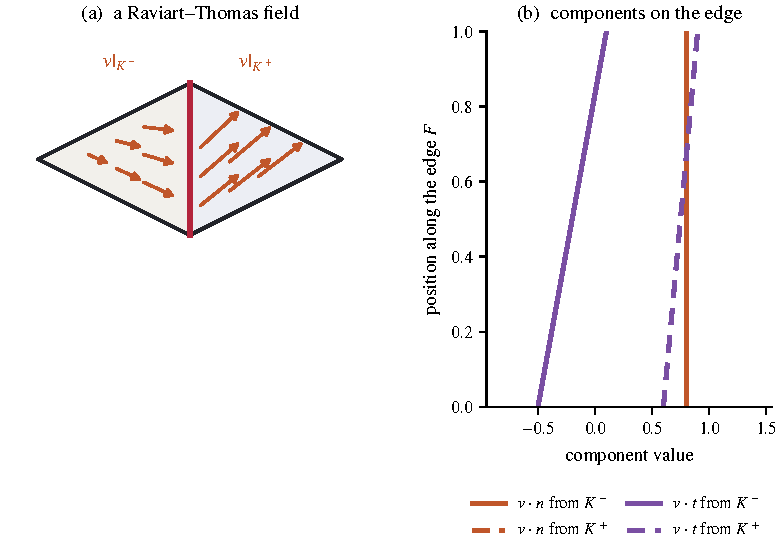
\includegraphics[width=\textwidth]{fig_rt_normal.pdf}
\caption{A Raviart--Thomas field on the two-cell patch. Left: the arrows visibly
kink as they cross the shared edge --- this is \emph{not} a continuous vector
field. Right: resolving the two one-sided traces into components along the edge
shows what is really going on. The two normal-component curves (orange, solid
from $K^-$ and dashed from $K^+$) lie exactly on top of one another, while the
two tangential curves (purple) are completely different functions.}
\label{fig:rt}
\end{figure}

\subsection{What normal continuity means physically}

Flux. The quantity $\int_F \bu\cdot\bn$ is the amount of fluid crossing the
facet $F$ per unit time. A jump in $\bu\cdot\bn$ would mean that the amount
leaving one cell differs from the amount entering the next --- mass appearing
or vanishing on a surface of zero volume.

Normal continuity therefore \emph{is} conservation, and in the discrete method
it is exact rather than approximate. Take $q = 1$ on a single cell $K$ and $0$
elsewhere in the second equation of \eqref{eq:mixed}; the divergence theorem
turns it into
\[
  \int_{\partial K} \bu_h \cdot \bn \ds \;=\; \int_K f \dx ,
\]
which holds to machine precision, on every cell, on every mesh, however coarse.
Reservoir and transport codes care about this a great deal: an ``accurate'' flow
field that leaks mass will corrupt the concentration field it is coupled to.

\begin{figure}[htbp]
\centering
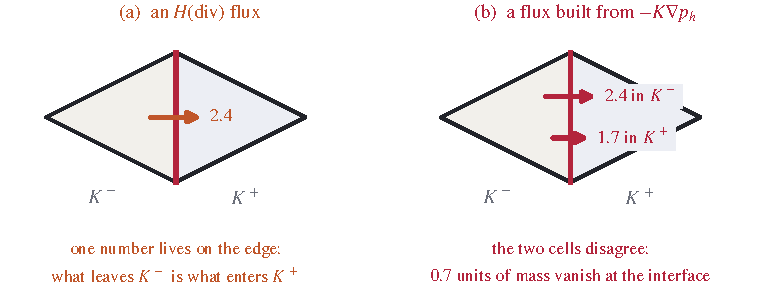
\includegraphics[width=\textwidth]{fig_conservation.pdf}
\caption{Local conservation. With an $\Hdiv$-conforming flux there is exactly
one flux value on the shared edge and it is shared by both cells. A flux
recovered by differentiating a continuous pressure, $-K\nabla p_h$, has two
different values on that edge --- and the difference is mass that the scheme
creates or destroys at the interface.}
\label{fig:conservation}
\end{figure}

\subsection{Why plain Lagrange elements are the wrong tool here}

Three independent reasons, each sufficient on its own.

\begin{enumerate}
\item \textbf{The physics has a tangential jump.} Suppose the permeability $K$
  jumps across a geological layer boundary, as it always does. The pressure $p$
  is continuous, so its tangential derivative along the interface is continuous,
  and therefore the tangential velocity $\bu\cdot\bt = -K\,\partial_t p$
  \emph{jumps} by the same ratio as $K$. Meanwhile $\bu\cdot\bn$ stays
  continuous, because mass is conserved. The true solution is thus normally
  continuous and tangentially discontinuous --- precisely an $\Hdiv$ field. A
  continuous vector Lagrange space forces \emph{both} components to match and
  cannot represent it; it will smear the layer over one cell and converge
  slowly or to the wrong thing.
\item \textbf{No local conservation.} A flux post-processed as $-K\nabla p_h$
  from a Lagrange pressure has two different values on each facet
  (Figure~\ref{fig:conservation}), so cellwise mass balance fails.
\item \textbf{Stability.} The mixed system \eqref{eq:mixed} is a saddle point
  problem, and not every pair of spaces gives an invertible system. $RT_k$
  paired with discontinuous $P_k$ is one of the classical stable pairs; obvious
  alternatives such as continuous $(P_1)^2$ with discontinuous $P_0$ are not.
  The inf-sup condition behind this is discussed in
  Section~\ref{sec:taylorhood}.
\end{enumerate}

\FloatBarrier

% =================================================================== \S 6 ==
\section{BDM: the same continuity, a different polynomial space}

\begin{keypoint}[cHdiv]
\textbf{Approximates:} the same thing as $RT$ --- a flux.\quad
\textbf{Continuous:} the same thing --- $\bv\cdot\bn$.\quad
\textbf{Lives in:} the same space --- $\Hdiv$.\quad
\textbf{Differs in:} which polynomials are kept, and therefore in the trade-off
between accuracy in $\bv$ and accuracy in $\dv\bv$.
\end{keypoint}

\subsection{The element}

The Brezzi--Douglas--Marini element takes the \emph{complete} polynomial space
of degree $k$,
\[
  BDM_k(K) = (P_k(K))^2, \qquad \dim BDM_k = (k+1)(k+2), \qquad k \ge 1,
\]
and imposes $\Hdiv$-conformity through the dofs rather than by restricting the
polynomials. The normal trace of a $(P_k)^2$ field on an edge is a full
polynomial of degree $k$ in one variable, so it takes $k+1$ dofs per edge to pin
it down:
\[
  \bv \;\longmapsto\; \int_{F} (\bv\cdot\bn)\, q \ds, \qquad q \in P_k(F).
\]
For $BDM_1$ that is $3 \times 2 = 6$ dofs, exactly $\dim (P_1)^2$, so the
lowest-order BDM element has no interior dofs at all.

\subsection{The essential difference from $RT$}

Both families are $\Hdiv$-conforming and both contain $(P_k)^2$. What separates
them is the \emph{divergence}:
\[
  \dv\, RT_k = P_k, \qquad\qquad \dv\, BDM_k = P_{k-1}.
\]
$RT_k$ was constructed by adding just enough extra to $(P_k)^2$ to make the
divergence surjective onto $P_k$; $BDM_k$ was not. The consequence for accuracy
is a genuine trade-off:

\begin{table}[htbp]
\centering
\small
\caption{Lowest orders on a triangle. Both $BDM_1$ and $RT_1$ approximate the
field itself to second order, but $BDM_1$ does it with six dofs instead of
eight --- at the price of one order in the divergence.}
\label{tab:rtbdm}
\begin{tabular}{@{}lccll@{}}
\toprule
Space & dofs & contains & $\|\bv - \bv_h\|_{L^2}$ & $\|\dv(\bv - \bv_h)\|_{L^2}$ \\
\midrule
$RT_0$   & 3 & $(P_0)^2$ & $O(h)$   & $O(h)$   \\
$BDM_1$  & 6 & $(P_1)^2$ & $O(h^2)$ & $O(h)$   \\
$RT_1$   & 8 & $(P_1)^2$ & $O(h^2)$ & $O(h^2)$ \\
\bottomrule
\end{tabular}
\end{table}

\subsection{When to prefer which}

\begin{description}
\item[Choose $RT_k$] when the divergence is part of the answer. If you need the
  mass balance resolved to the same order as the velocity --- for instance when
  $f$ is not piecewise constant and you want $\dv \bu_h$ to track it
  accurately --- the balanced approximation of $RT$ is what you want. It pairs
  naturally with discontinuous $P_k$ for the scalar unknown.
\item[Choose $BDM_k$] when you want the best field accuracy per degree of
  freedom. $BDM_1$ delivers the same $O(h^2)$ velocity as $RT_1$ from a smaller
  system. It pairs with discontinuous $P_{k-1}$.
\item[In elasticity,] where the unknown is a stress \emph{tensor}, $BDM$ rows
  are the standard building block: each row of the stress is an $\Hdiv$ vector
  field, because the equilibrium equation $\dv\sigma = -f$ applies the
  divergence row by row. The companion repository to this guide uses exactly
  this construction (Section~\ref{sec:falk}).
\end{description}

There is also a structural way to say the difference, which
Section~\ref{sec:derham} will make precise: $BDM$ is the \emph{full} polynomial
family and $RT$ is the \emph{trimmed} one. They are the two natural members of
the same construction, not rivals.

\FloatBarrier

% =================================================================== \S 7 ==
\section{Nédélec elements: gluing the tangential component}
\label{sec:nedelec}

\begin{keypoint}[cHcurl]
\textbf{Approximates:} an electromagnetic field.\quad
\textbf{Dofs:} circulations along edges.\quad
\textbf{Continuous:} the tangential component.\quad
\textbf{Lives in:} $\Hcurl$.\quad
\textbf{Used for:} Maxwell's equations, eddy currents, waveguides, cavity
resonances.
\end{keypoint}

\subsection{The problem that demands it}

The time-harmonic Maxwell system, after eliminating the magnetic field, reads
\[
  \curl\!\big(\mu^{-1} \curl \bE\big) \;-\; \omega^2 \varepsilon\, \bE
  \;=\; \mathbf{J},
\]
and its weak form is
\[
  \int_\Omega \mu^{-1} (\curl \bE)\cdot(\curl \mathbf{F}) \dx
  \;-\; \omega^2 \int_\Omega \varepsilon\, \bE \cdot \mathbf{F} \dx
  \;=\; \int_\Omega \mathbf{J}\cdot\mathbf{F} \dx .
\]
Every derivative enters through $\curl$. By the rule of Section~2 the field
belongs in $\Hcurl$, and the conforming discrete space must have continuous
tangential components --- nothing more.

\subsection{The element}

In two dimensions the lowest-order Nédélec element of the first kind is the
$90^\circ$ rotation of $RT_0$:
\[
  N_0(K) = \big\{\, \bv(\bx) = \mathbf{a} + b\,\bx^{\perp} \,\big\},
  \qquad \bx^\perp = (-x_2,\, x_1),
\]
with the three dofs
\[
  \bv \;\longmapsto\; \int_{F_i} \bv \cdot \bt_i \ds .
\]
The same one-line miracle applies, rotated: along a straight edge the term
$b\,\bx^{\perp}$ has constant tangential component, so the tangential trace on
each edge is a single shared number.

In three dimensions this becomes the \emph{Whitney edge element}: one degree of
freedom per mesh edge, equal to the circulation $\int_e \bE\cdot\bt$ of the
field along that edge. On a tetrahedron that is six dofs. The name ``edge
element'' comes from exactly this --- the unknowns live on edges, not on
vertices.

\begin{figure}[htbp]
\centering
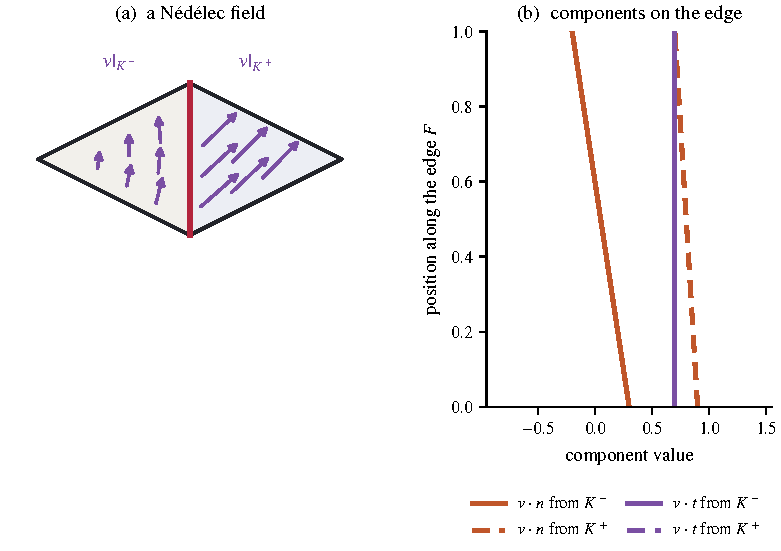
\includegraphics[width=\textwidth]{fig_nedelec_tangential.pdf}
\caption{A Nédélec field on the same patch. Compare with
Figure~\ref{fig:rt}: now it is the two \emph{tangential} curves (purple) that
coincide, while the two \emph{normal} curves (orange) are different functions.
The roles of the components are exactly swapped.}
\label{fig:nedelec}
\end{figure}

\subsection{What tangential continuity means physically}

Maxwell's interface conditions say it directly. Across a boundary between two
materials:
\begin{itemize}
\item the \emph{tangential} component of $\bE$ is continuous (this is Faraday's
  law applied to a vanishingly thin loop straddling the interface);
\item the \emph{normal} component of $\bE$ \emph{jumps}, by the ratio of the
  permittivities, whenever surface charge is present.
\end{itemize}
An $\Hcurl$-conforming element reproduces both statements exactly: it glues what
physics glues and leaves free what physics leaves free.

\subsection{Why Lagrange elements fail here --- and they really do fail}

This is the sharpest example in the guide of over-gluing causing actual damage.
Discretising $\bE$ with continuous vector Lagrange elements is not merely
suboptimal; it produces wrong answers.

\begin{enumerate}
\item \textbf{It forbids a jump the physics requires.} At a dielectric
  interface the normal component must jump. A continuous vector space forces it
  to be continuous, so the discrete solution cannot approach the true one near
  any material interface.
\item \textbf{Spurious modes.} Computing cavity resonances with nodal elements
  produces extra, entirely non-physical eigenvalues scattered through the
  spectrum, which are hard to distinguish from real ones. The cause is
  structural: the operator $\curl$ has a huge kernel (every gradient), and a
  stable discretisation must reproduce the relation ``curl-free $=$ gradient''
  exactly at the discrete level. Nédélec spaces do, because
  $\nabla(P_k\text{ Lagrange}) \subset N_{k-1}$ exactly. Nodal vector spaces do
  not, and the mismatch surfaces as spurious eigenvalues.
\item \textbf{Re-entrant corners.} Near a re-entrant corner or an edge of a
  conductor the true field is singular: it lies in $\Hcurl$ but not in
  $(H^1)^d$. A nodal method searches for its solution inside $(H^1)^d$, which
  does not contain the answer, and converges confidently to the wrong
  function.
\end{enumerate}

Point~2 is not a curiosity --- it is the historical reason edge elements were
invented, and it is the clearest illustration of the theme of
Section~\ref{sec:derham}: these element families are not an arbitrary
collection, and using the wrong one breaks a structure you did not know you
were relying on.

\FloatBarrier

% =================================================================== \S 8 ==
\section{Four more elements worth knowing}

\subsection{Crouzeix--Raviart: continuity at one point per edge}

The Crouzeix--Raviart element uses $P_1$ on each triangle, but places its three
dofs at the \emph{edge midpoints} rather than the vertices.

Two neighbouring cells now share one number per shared edge, not two. One number
is not enough to determine a linear trace, so the traces from the two sides
generally differ: the function is continuous at the midpoint of each edge and
nowhere else along it. The global space is therefore \emph{not} contained in
$H^1$.

\begin{jargon}{Nonconforming methods}
A method is \emph{nonconforming} when $V_h \not\subset V$ --- the discrete
functions are not legal candidates for the continuous problem at all. This
sounds fatal but is not, provided the violation shrinks fast enough under
refinement. For Crouzeix--Raviart the saving grace is that, because the midpoint
value of a linear function equals its average over the edge,
\[
  \int_F \jump{u_h} \ds = 0 \quad\text{on every edge } F,
\]
so the jump has zero mean even though it is not zero. That is exactly enough for
the consistency error to be $O(h)$ and the method to converge.
\end{jargon}

Why bother? Because this weaker gluing is precisely what some problems want:

\begin{itemize}
\item The pair (Crouzeix--Raviart velocity, piecewise constant pressure) is
  inf-sup stable for Stokes and remarkably cheap --- an attractive combination
  that no low-order \emph{conforming} pair achieves.
\item In nearly incompressible elasticity, conforming low-order elements suffer
  \emph{locking}: the incompressibility constraint uses up so many of the
  available degrees of freedom that the computed displacement is far too stiff.
  The extra freedom in the nonconforming space relieves this.
\end{itemize}

\subsection{Hermite and Argyris: when $H^1$ is not enough}

Fourth-order equations change the requirements entirely. For the biharmonic
equation $\Delta^2 w = f$ --- the model for the bending of a thin plate --- the
weak form pairs \emph{second} derivatives:
\[
  \int_\Omega D^2 w : D^2 v \dx = \int_\Omega f v \dx .
\]
Now the solution must live in $H^2$, and running the jump calculation of
Section~2 one order higher shows that a piecewise polynomial is in $H^2$ if and
only if \emph{both} the function and its normal derivative are continuous across
every facet --- that is, if and only if it is $C^1$.

Building $C^1$ piecewise polynomials on triangles is genuinely hard, and it is
easy to be misled:

\begin{description}
\item[The Hermite cubic triangle] has 10 dofs: the value and both first
  derivatives at each of the three vertices, plus the value at the centroid.
  Despite carrying derivative dofs it is only $C^0$: along a shared edge the two
  cells agree on the value and on the gradient \emph{at the two endpoints}, but
  the normal derivative varies quadratically along the edge and the endpoint
  data do not determine it. Hermite triangles are therefore \emph{not}
  $H^2$-conforming --- a common misconception worth stating plainly.
\item[The Argyris triangle] does the job. It uses quintic polynomials, with 21
  dofs: at each vertex the value, both first derivatives and all three second
  derivatives ($6 \times 3 = 18$), plus the normal derivative at each edge
  midpoint ($3$). Since $\dim P_5 = 21$, this is unisolvent, and the resulting
  space really is $C^1$ and $H^2$-conforming. It is expensive, and it is
  awkward on curved boundaries, but it is correct.
\end{description}

In practice many codes sidestep $C^1$ entirely --- by rewriting the fourth-order
problem as a mixed system of two second-order ones, or by using a $C^0$ interior
penalty method that enforces normal-derivative continuity weakly, in the spirit
of Section~4.

\subsection{Taylor--Hood: elements come in pairs}
\label{sec:taylorhood}

The Stokes equations describe slow viscous flow:
\[
  -\nu \Delta \bu + \nabla p = \mathbf{f}, \qquad \dv \bu = 0 .
\]
There are two unknowns, so there are two discrete spaces, and the new
difficulty is that they must be chosen \emph{together}. Here the pressure acts
as a Lagrange multiplier enforcing $\dv\bu = 0$, and a multiplier space can be
too rich for the space it constrains.

\begin{jargon}{The inf-sup (LBB) condition}
A mixed pair $(V_h, Q_h)$ is stable if there is a constant $\beta > 0$,
independent of $h$, with
\[
  \inf_{q_h \in Q_h}\ \sup_{\bv_h \in V_h}\
  \frac{\displaystyle\int_\Omega q_h \dv \bv_h \dx}
       {\|\bv_h\|_{H^1}\, \|q_h\|_{L^2}} \;\ge\; \beta .
\]
In words: for every possible pressure there must exist a velocity that
``notices'' it. If some nonzero $q_h$ is invisible to every velocity in $V_h$,
the discrete system has a spurious pressure mode and the computed pressure is
garbage --- even though the velocity may look fine.
\end{jargon}

The classical failure is equal-order $P_1$/$P_1$, which admits a checkerboard
pressure: a pattern alternating $+1$ and $-1$ from cell to cell that the
discrete divergence simply cannot see. The Taylor--Hood pair, $P_2$ velocity with
continuous $P_1$ pressure, is inf-sup stable, and is the standard workhorse for
incompressible flow.

\begin{figure}[htbp]
\centering
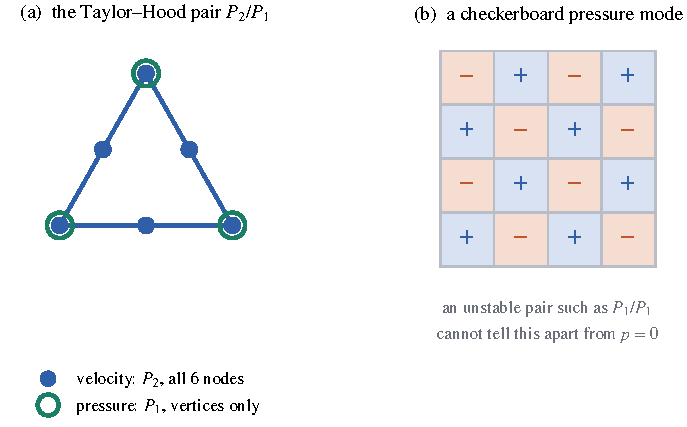
\includegraphics[width=\textwidth]{fig_taylor_hood.pdf}
\caption{The Taylor--Hood pair: velocity dofs at all six $P_2$ nodes, pressure
dofs at the three vertices only. Right: the checkerboard mode that destroys
equal-order pairs. A stable pair must be rich enough in velocity to detect
every pressure pattern.}
\label{fig:th}
\end{figure}

This is the same requirement met earlier in disguise. $RT_k$ with discontinuous
$P_k$, and $BDM_k$ with discontinuous $P_{k-1}$, are stable pairs for the mixed
Poisson problem \eqref{eq:mixed} for exactly this reason. Pairing spaces is not
guesswork; it is what the next section is about.

\FloatBarrier

% =================================================================== \S 9 ==
\clearpage
\section{One table for all of them}

\begin{table}[htbp]
\centering
\footnotesize
\setlength{\tabcolsep}{4.2pt}
\renewcommand{\arraystretch}{1.28}
\caption{The families at a glance. ``Continuous quantity'' is the single most
useful column: it is what distinguishes the families, and everything else
follows from it.}
\label{tab:all}
\begin{tabular}{@{}>{\raggedright\arraybackslash}p{2.25cm}
                  >{\raggedright\arraybackslash}p{1.25cm}
                  >{\raggedright\arraybackslash}p{1.35cm}
                  >{\raggedright\arraybackslash}p{2.6cm}
                  >{\raggedright\arraybackslash}p{2.85cm}
                  >{\raggedright\arraybackslash}p{2.7cm}@{}}
\toprule
\textbf{Element} & \textbf{Scalar / vector} & \textbf{Global space} &
\textbf{Continuous quantity} & \textbf{Typical dofs} & \textbf{Typical PDE} \\
\midrule

\cH{Lagrange $P_k$} & scalar & $H^1$ &
the whole value & point values at vertices, edge and interior nodes &
Poisson, heat, elasticity \\

\textcolor{cCR}{Crouzeix--Raviart} & scalar & \emph{none} (nonconforming) &
value at edge midpoints only; jump has zero mean &
value at each edge midpoint &
Stokes, incompressible elasticity \\

\cL{Discontinuous $P_k$} & either & $L^2$ &
nothing & cell-local nodal values &
transport, conservation laws, mixed methods \\

\cD{$RT_k$} & vector & $\Hdiv$ &
normal component $\bv\cdot\bn$ &
normal moments on facets $+$ interior moments &
Darcy, mixed Poisson \\

\cD{$BDM_k$} & vector & $\Hdiv$ &
normal component $\bv\cdot\bn$ &
$k+1$ normal moments per facet &
mixed Poisson, stress in elasticity \\

\cC{Nédélec $N_k$} & vector & $\Hcurl$ &
tangential component &
circulations along edges &
Maxwell, eddy currents, waveguides \\

\textcolor{cInk}{Argyris $P_5$} & scalar & $H^2$ &
value \emph{and} normal derivative &
value, gradient, Hessian at vertices; normal derivative at edge midpoints &
biharmonic, plate bending \\

\cH{Taylor--Hood} & pair & $H^1 \times H^1$ &
both values; stable by inf-sup &
$P_2$ velocity nodes, $P_1$ pressure vertices &
Stokes, Navier--Stokes \\

\bottomrule
\end{tabular}
\end{table}

\FloatBarrier

% ================================================================== \S 10 ==
\section{The de Rham complex: why this is a family, not a list}
\label{sec:derham}

Everything so far could be read as a catalogue of unrelated tricks: someone
needed normal continuity and invented $RT$; someone else needed tangential
continuity and invented Nédélec. That reading is wrong, and this section is the
most important one in the guide.

\subsection{The sequence}

Consider the three classical differential operators of vector calculus in three
dimensions, arranged in order:
\[
  H^1 \;\xrightarrow{\ \operatorname{grad}\ }\;
  \Hcurl \;\xrightarrow{\ \curl\ }\;
  \Hdiv \;\xrightarrow{\ \dv\ }\;
  L^2 .
\]
Each space is exactly the natural domain of the operator leaving it, and the
image of each operator lands inside the domain of the next. Two identities you
already know make the composition of consecutive arrows vanish:
\[
  \curl\,(\operatorname{grad} \phi) = 0, \qquad \dv\,(\curl \bv) = 0 .
\]
More than that: on a domain without holes the converses hold too. A curl-free
field \emph{is} a gradient; a divergence-free field \emph{is} a curl. In other
words, at each stage the image of one arrow is \emph{exactly} the kernel of the
next. A sequence with that property is called \emph{exact}, and this particular
one is the \emph{de Rham complex}.

Read physically, it is a chain of familiar facts: a potential has a field; a
field has a flux; a flux has a source density.

\subsection{The discrete copy}

Here is the point. The finite element families in this guide form a discrete
sequence with the \emph{same} structure:
\[
  \underbrace{P_k}_{\cH{\text{Lagrange}}}
  \;\xrightarrow{\ \operatorname{grad}\ }\;
  \underbrace{N_{k-1}}_{\cC{\text{Nédélec}}}
  \;\xrightarrow{\ \curl\ }\;
  \underbrace{RT_{k-1}}_{\cD{\text{Raviart--Thomas}}}
  \;\xrightarrow{\ \dv\ }\;
  \underbrace{P_{k-1}}_{\cL{\text{discontinuous}}} .
\]
The gradient of a continuous piecewise polynomial really does land in the
Nédélec space; the curl of a Nédélec function really does land in
Raviart--Thomas; the divergence of a Raviart--Thomas function really does land
in the discontinuous space --- and the exactness property survives
discretisation intact.

\begin{figure}[htbp]
\centering
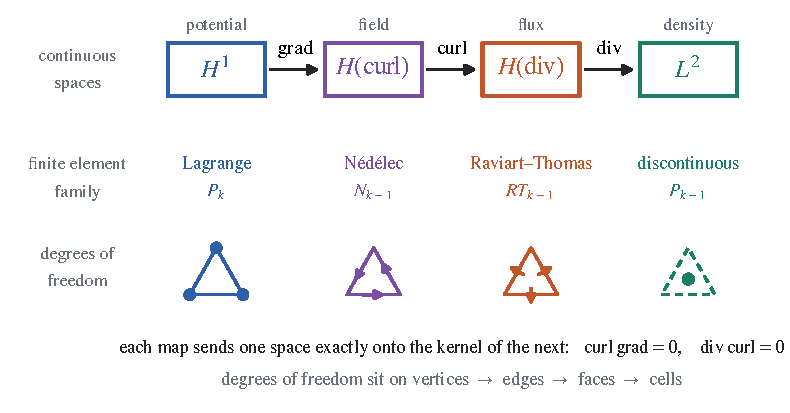
\includegraphics[width=\textwidth]{fig_derham.pdf}
\caption{The de Rham complex and its finite element realisation. Top: the
continuous spaces and the operators linking them. Middle: the element family
occupying each slot. Bottom: where the degrees of freedom sit --- vertices,
then edges, then faces, then cell interiors. The four families of this guide
are the four slots of one sequence.}
\label{fig:derham}
\end{figure}

Notice the bottom row of Figure~\ref{fig:derham}: the dofs march from vertices
to edges to faces to cell interiors as you move along the sequence. That is not
a coincidence either. In the language of differential forms, the four families
are the finite element versions of $0$-forms, $1$-forms, $2$-forms and
$3$-forms, and a $p$-form is naturally integrated over a $p$-dimensional piece
of the mesh. Point values on vertices, circulations along edges, fluxes through
faces, densities over cells.

\subsection{What exactness buys}

\begin{itemize}
\item \textbf{No spurious modes.} The Maxwell eigenvalue problem is well
  behaved precisely because the discrete kernel of $\curl$ equals the discrete
  gradients --- which is discrete exactness at the second arrow. This is the
  structural reason behind Section~\ref{sec:nedelec}, point~2.
\item \textbf{Stable mixed methods.} The inf-sup condition of
  Section~\ref{sec:taylorhood} for the pair $RT_k \times P_k$ follows from the
  divergence being surjective onto the discontinuous space --- exactness at the
  third arrow. Choosing spaces from the same complex is a recipe for stability
  rather than a matter of luck.
\item \textbf{Commuting interpolation.} Interpolating a function and then
  differentiating gives the same result as differentiating and then
  interpolating. Many error estimates fall out of this one diagram.
\end{itemize}

\subsection{Two complexes in two dimensions, and where $BDM$ sits}

In two dimensions the sequence splits into two shorter ones, because $\curl$
has two different two-dimensional analogues:
\[
  H^1 \xrightarrow{\ \operatorname{curl}\ } \Hdiv \xrightarrow{\ \dv\ } L^2,
  \qquad\qquad
  H^1 \xrightarrow{\ \operatorname{grad}\ } \Hcurl \xrightarrow{\ \operatorname{rot}\ } L^2,
\]
where $\operatorname{curl}\phi = (\partial_y \phi, -\partial_x \phi)$ is the
rotated gradient and $\operatorname{rot}\bv = \partial_x v_2 - \partial_y v_1$
is the scalar curl. The second is the first with everything rotated by
$90^\circ$ --- which is exactly the relationship between $N_0$ and $RT_0$ noted
in Section~\ref{sec:nedelec}.

Finally, $BDM$. The modern account, \emph{finite element exterior calculus},
shows that each slot of the complex admits \emph{two} natural polynomial
families: a \emph{trimmed} one and a \emph{full} one. $RT$ and Nédélec of the
first kind are the trimmed family; $BDM$ and Nédélec of the second kind are the
full family. Table~\ref{tab:rtbdm} was an instance of that general pattern, and
it explains why the trade-off there looked so systematic.

\begin{keypoint}[cInk]
This framework is due to Arnold, Falk and Winther. The same Richard Falk gives
his name to the mixed elasticity element implemented in the companion
repository --- which is, as the next section shows, an application of exactly
this way of thinking.
\end{keypoint}

\FloatBarrier

% ================================================================== \S 11 ==
\section{Putting it together}

\subsection{A worked example: one element, three spaces}
\label{sec:falk}

The repository accompanying these notes solves linear elasticity in mixed form
with weakly imposed symmetry, using the element introduced by Falk. It has three
unknowns, and --- the point of this guide in miniature --- each one lives in a
different tier of the hierarchy.

\begin{figure}[htbp]
\centering
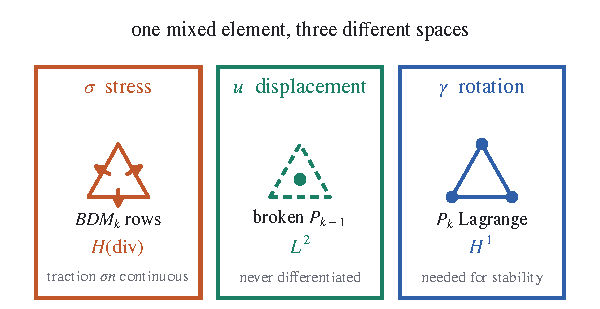
\includegraphics[width=0.94\textwidth]{fig_falk.pdf}
\caption{The three fields of the Falk mixed element, and the space each one
needs. Reading the weak form tells you which is which.}
\label{fig:falk}
\end{figure}

\begin{description}
\item[The stress $\sigma$ sits in $\Hdiv$.] The equilibrium equation
  $\dv\sigma = -f$ applies the divergence to each row of the stress tensor, so
  each row must be an $\Hdiv$ vector field --- in this implementation, a $BDM_k$
  field. The physical content of normal continuity here is Newton's third law:
  the traction $\sigma\bn$ that one side of an interface exerts on the other is
  equal and opposite, so it cannot jump.
\item[The displacement $u$ sits in $L^2$.] In the mixed form the displacement is
  never differentiated --- the derivative has been moved onto the stress. By the
  logic of Section~4 there is no reason to ask for continuity, so $u$ is a
  broken (discontinuous) $P_{k-1}$ field.
\item[The rotation $\gamma$ sits in $H^1$.] This is the Lagrange multiplier
  enforcing the symmetry $\sigma = \sigma^{\!\top}$, and it is the subtle one:
  it is not differentiated either, yet it needs full $H^1$ continuity. The
  reason is stability, not regularity --- the inf-sup argument for this element
  routes through a Stokes-like pairing that fails if the multiplier space is
  taken any larger.
\end{description}

That last point is a useful corrective to a rule stated too simply. ``No
derivative, no continuity'' is the right first instinct, but stability can
demand more, and in a mixed method the spaces must always be checked as a
system rather than one at a time.

\subsection{How to choose, in practice}

\begin{enumerate}
\item \textbf{Write down the weak form first.} Not the PDE --- the weak form.
  Integrate by parts the way you actually intend to, and see which derivative
  survives on which unknown.
\item \textbf{Match the space to the surviving derivative.} Full gradient
  $\Rightarrow$ $H^1$ $\Rightarrow$ Lagrange. Only $\dv$ $\Rightarrow$ $\Hdiv$
  $\Rightarrow$ $RT$ or $BDM$. Only $\curl$ $\Rightarrow$ $\Hcurl$
  $\Rightarrow$ Nédélec. No derivative $\Rightarrow$ $L^2$ $\Rightarrow$
  discontinuous.
\item \textbf{Ask what the true solution does at material interfaces.} If a
  component genuinely jumps there, any space that forbids the jump is
  disqualified regardless of what the derivative count said.
\item \textbf{For several unknowns, check the pair, not the pieces.} Take the
  spaces from one de Rham complex where you can; otherwise verify the inf-sup
  condition or use a documented stable pair.
\item \textbf{Then, and only then, pick a degree.} Higher $k$ pays off when the
  solution is smooth; near corners and interfaces, mesh refinement is usually
  the better investment.
\end{enumerate}

\subsection{The one-page summary}

\begin{figure}[htbp]
\centering
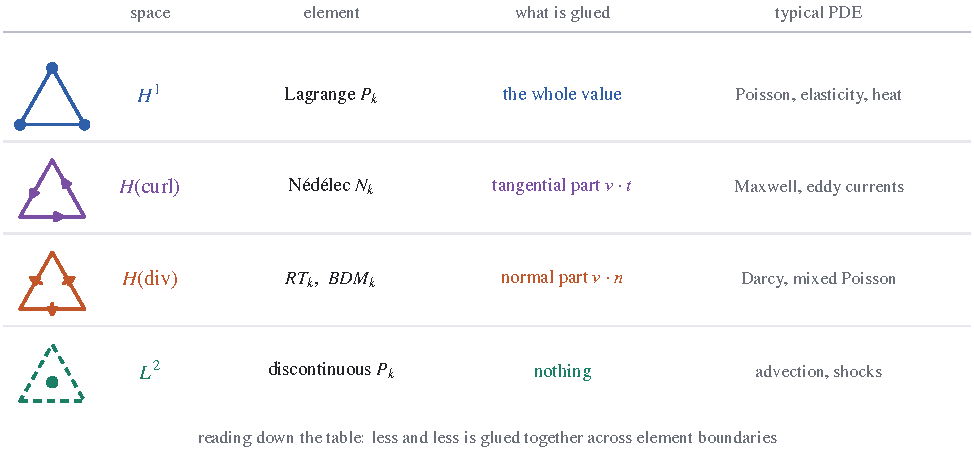
\includegraphics[width=\textwidth]{fig_cheatsheet.pdf}
\caption{The whole guide in one picture. Reading down: less and less is glued
across element boundaries, the space gets larger, and the method asks less of
the solution. The right element is the one that glues exactly what the equation
--- and the physics --- says should be glued, and not one bit more.}
\label{fig:cheat}
\end{figure}

\begin{figure}[htbp]
\centering
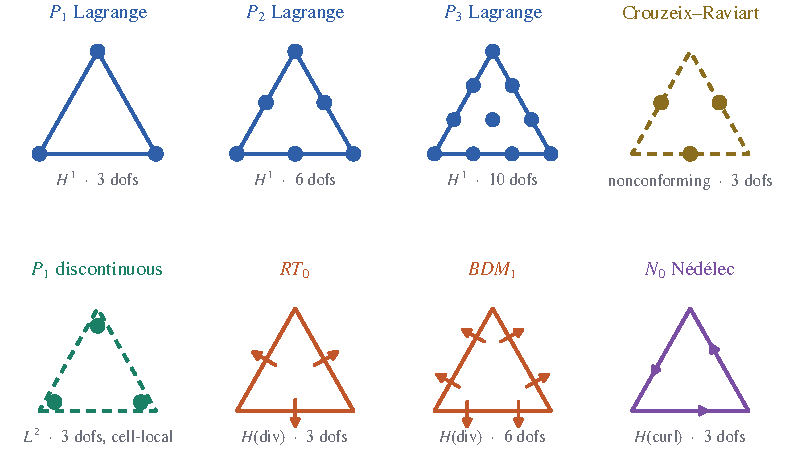
\includegraphics[width=\textwidth]{fig_dof_zoo.pdf}
\caption{Degrees of freedom on the reference triangle. Filled circles are point
values; arrows across an edge are normal moments; arrows along an edge are
tangential moments; a dashed outline means nothing is shared with the
neighbours. The position of the markers is the whole story: dofs on shared
vertices and edges create continuity, dofs in the interior do not.}
\label{fig:zoo}
\end{figure}

\FloatBarrier

\section*{Where to go next}
\addcontentsline{toc}{section}{Where to go next}

\begin{description}
\item[Run the demonstration.] The script \texttt{examples/visualize\_elements.py}
  in this directory draws the four behaviours of Figures~\ref{fig:lagrange},
  \ref{fig:dgjump}, \ref{fig:rt} and~\ref{fig:nedelec} from explicitly
  constructed basis functions, with every space written out in a few lines of
  numpy. Reading it is a good way to convince yourself that nothing here is
  magic. See \texttt{README.md} for how to run it.
\item[Standard references.] Brenner \& Scott, \emph{The Mathematical Theory of
  Finite Element Methods}, for the general framework; Boffi, Brezzi \& Fortin,
  \emph{Mixed Finite Element Methods and Applications}, for everything mixed;
  Arnold, Falk \& Winther, \emph{Finite element exterior calculus}
  (Acta Numerica, 2006), for the structure of Section~\ref{sec:derham};
  Monk, \emph{Finite Element Methods for Maxwell's Equations}, for edge
  elements.
\item[In software.] The DefElement project catalogues these elements with
  explicit basis functions and consistent conventions, and is the fastest way
  to check a definition or a dof count.
\end{description}

\end{document}
